\tikzset{every picture/.style={line width=0.75pt}} %set default line width to 0.75pt        

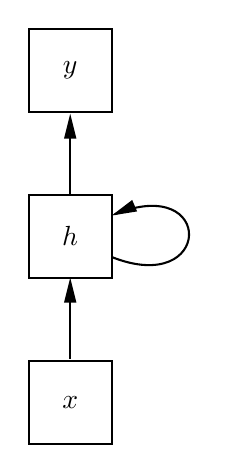
\begin{tikzpicture}[x=0.75pt,y=0.75pt,yscale=-1,xscale=1]
%uncomment if require: \path (0,300); %set diagram left start at 0, and has height of 300

%Shape: Square [id:dp8692809145396877] 
\draw   (90,160) -- (130,160) -- (130,200) -- (90,200) -- cycle ;
%Shape: Square [id:dp38928267638281655] 
\draw   (90,80) -- (130,80) -- (130,120) -- (90,120) -- cycle ;
%Shape: Square [id:dp3868167754548386] 
\draw   (90,240) -- (130,240) -- (130,280) -- (90,280) -- cycle ;
%Straight Lines [id:da760409127154227] 
\draw    (110,239) -- (110,202) ;
\draw [shift={(110,200)}, rotate = 90] [fill={rgb, 255:red, 0; green, 0; blue, 0 }  ][line width=0.08]  [draw opacity=0] (12,-3) -- (0,0) -- (12,3) -- cycle    ;
%Straight Lines [id:da541971324827849] 
\draw    (110,160) -- (110,123) ;
\draw [shift={(110,121)}, rotate = 90] [fill={rgb, 255:red, 0; green, 0; blue, 0 }  ][line width=0.08]  [draw opacity=0] (12,-3) -- (0,0) -- (12,3) -- cycle    ;
%Curve Lines [id:da7501561975230205] 
\draw    (130,190) .. controls (178.68,209.31) and (180.14,149.71) .. (131.49,169.38) ;
\draw [shift={(130,170)}, rotate = 336.8] [fill={rgb, 255:red, 0; green, 0; blue, 0 }  ][line width=0.08]  [draw opacity=0] (12,-3) -- (0,0) -- (12,3) -- cycle    ;

% Text Node
\draw (110,260) node   [align=left] {$\displaystyle x$};
% Text Node
\draw (110,180) node   [align=left] {$\displaystyle h$};
% Text Node
\draw (110,100) node   [align=left] {$\displaystyle y$};


\end{tikzpicture}